\section{Parallele Modelle}

%----------------------------------------------------------------------%SLIDE -
\begin{frame}
    \frametitle{Parallele Modelle}
    \tableofcontents[
        currentsection,
        hideothersubsections,
        sectionstyle=show/hide,
    ]
\end{frame}
%----------------------------------------------------------------------%SLIDE -


\subsection{Circuit}
%----------------------------------------------------------------------%SLIDE -
\begin{frame}
    \frametitle{Circuit}
    \begin{columns}
        \begin{column}{0.5\textwidth}
            \begin{itemize}
                \item gerichteter, azyklischer Graph (DAG)
                \item Eingabe, Ausgabe
                \item Operationen
                \item Boolean Circuit
                \item interessant für theoretische Überlegungen
            \end{itemize}
        \end{column}
        \begin{column}{0.5\textwidth}
            \begin{figure}
                \centering
                % sequential circuit computing the sum of eight numbers
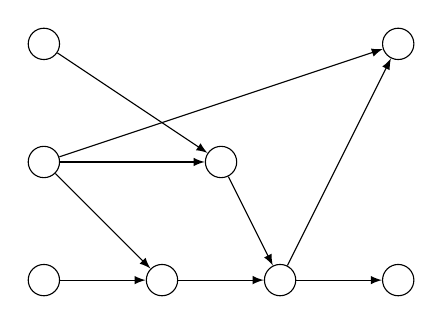
\begin{tikzpicture}
    [
        vertex/.style={circle, scale=1.2, draw,},
        edge/.style={-latex,},
        scale=1.5,
    ]

    % sequential dag
    \node (1) at (0,0)    [vertex] {};
    \node (2) at (0,1)    [vertex] {};
    \node (3) at (0,2)    [vertex] {};
    \node (4) at (1,0)    [vertex] {};
    \node (5) at (1.5,1)    [vertex] {};
    \node (6) at (2,0)    [vertex] {};
    \node (7) at (3,0)    [vertex] {};
    \node (8) at (3,2)    [vertex] {};

    \draw [edge] (1) -- (4);
    \draw [edge] (2) -- (4);
    \draw [edge] (2) -- (5);
    \draw [edge] (2) -- (8);
    \draw [edge] (3) -- (5);
    \draw [edge] (4) -- (6);
    \draw [edge] (5) -- (6);
    \draw [edge] (6) -- (7);
    \draw [edge] (6) -- (8);

\end{tikzpicture}         

                \caption{Ein DAG}
                \label{fig:dag}
            \end{figure}
        \end{column}
    \end{columns}
\end{frame}
%----------------------------------------------------------------------%SLIDE -

%----------------------------------------------------------------------%SLIDE -
\begin{frame}[b]
    \frametitle{Boolean Circuit}
    \framesubtitle{Addition von acht Zahlen}
    \begin{columns}[b]
        \column{0.5\textwidth}
        \begin{figure}
            \centering
            % sequential circuit computing the sum of eight numbers
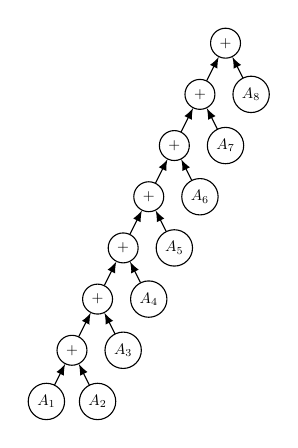
\begin{tikzpicture}
    [
        vertex/.style={circle, draw, scale=0.55, minimum size=3ex,},
        edge/.style={-latex,},
        scale=0.65,
    ]

    % sequential dag
    \node (b1) at (-3,0)    [vertex] {$A_1$};
    \node (b2) at (-2,0)    [vertex] {$A_2$};

    \node (q1) at (-2.5,1)  [vertex] {$+$};
    \node (b3) at (-1.5,1)  [vertex] {$A_3$};

    \node (q2) at (-2,2)    [vertex] {$+$};
    \node (b4) at (-1,2)    [vertex] {$A_4$};

    \node (q3) at (-1.5,3)  [vertex] {$+$};
    \node (b5) at (-0.5,3)  [vertex] {$A_5$};

    \node (q4) at (-1,4)    [vertex] {$+$};
    \node (b6) at (0,4)     [vertex] {$A_6$};

    \node (q5) at (-0.5,5)  [vertex] {$+$};
    \node (b7) at (0.5,5)   [vertex] {$A_7$};

    \node (q6) at (0,6)     [vertex] {$+$};
    \node (b8) at (1,6)     [vertex] {$A_8$};

    \node (q7) at (0.5,7)   [vertex] {$+$};

    \draw [edge] (b1) -- (q1);
    \draw [edge] (b2) -- (q1);
    \draw [edge] (b3) -- (q2);
    \draw [edge] (b4) -- (q3);
    \draw [edge] (b5) -- (q4);
    \draw [edge] (b6) -- (q5);
    \draw [edge] (b7) -- (q6);
    \draw [edge] (b8) -- (q7);
    \draw [edge] (q1) -- (q2);
    \draw [edge] (q2) -- (q3);
    \draw [edge] (q3) -- (q4);
    \draw [edge] (q4) -- (q5);
    \draw [edge] (q5) -- (q6);
    \draw [edge] (q6) -- (q7);

\end{tikzpicture}         

            \caption{eine Möglichkeit}
        \end{figure}
        \pause
        \column{0.5\textwidth}
        \begin{figure}
            \centering
            % parallel circuit computing the sum of eight numbers
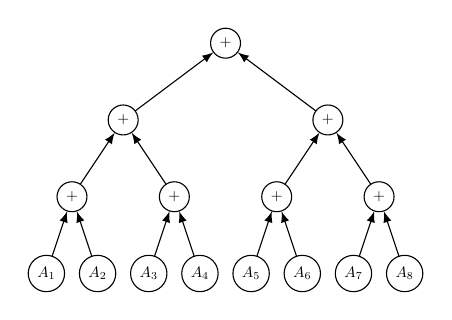
\begin{tikzpicture}
    [
        vertex/.style={circle, draw, scale=0.55, minimum size=3ex,},
        edge/.style={-latex,},
        scale=0.65,
    ]

    % parallel dag
    \node (a1) at (0,0)     [vertex] {$A_1$};
    \node (a2) at (1,0)     [vertex] {$A_2$};
    \node (a3) at (2,0)     [vertex] {$A_3$};
    \node (a4) at (3,0)     [vertex] {$A_4$};
    \node (a5) at (4,0)     [vertex] {$A_5$};
    \node (a6) at (5,0)     [vertex] {$A_6$};
    \node (a7) at (6,0)     [vertex] {$A_7$};
    \node (a8) at (7,0)     [vertex] {$A_8$};
    \node (p1) at (0.5,1.5) [vertex] {$+$};
    \node (p2) at (2.5,1.5) [vertex] {$+$};
    \node (p3) at (4.5,1.5) [vertex] {$+$};
    \node (p4) at (6.5,1.5) [vertex] {$+$};
    \node (p5) at (1.5,3)   [vertex] {$+$};
    \node (p6) at (5.5,3)   [vertex] {$+$};
    \node (p7) at (3.5,4.5) [vertex] {$+$};
    \draw [edge] (a1) -- (p1);
    \draw [edge] (a2) -- (p1);
    \draw [edge] (a3) -- (p2);
    \draw [edge] (a4) -- (p2);
    \draw [edge] (a5) -- (p3);
    \draw [edge] (a6) -- (p3);
    \draw [edge] (a7) -- (p4);
    \draw [edge] (a8) -- (p4);
    \draw [edge] (p1) -- (p5);
    \draw [edge] (p2) -- (p5);
    \draw [edge] (p3) -- (p6);
    \draw [edge] (p4) -- (p6);
    \draw [edge] (p5) -- (p7);
    \draw [edge] (p6) -- (p7);

\end{tikzpicture}         

            \caption{eine andere}
        \end{figure}
    \end{columns}
\end{frame}
%----------------------------------------------------------------------%SLIDE -

\subsection{Netzwerk}
%----------------------------------------------------------------------%SLIDE -
\begin{frame}
    \frametitle{Netzwerk}
    \begin{columns}
        \column{0.5\textwidth}
        \begin{itemize}
            \item \emph{distributed memory} Modell
            \item ungerichteter Graph
            \item RAMs
            \item feste Verbindungen
            \item verschiedene Topologien
            \item \textbf{send} und \textbf{receive}
        \end{itemize}
        \column{0.5\textwidth}
        \begin{figure}
            \centering
            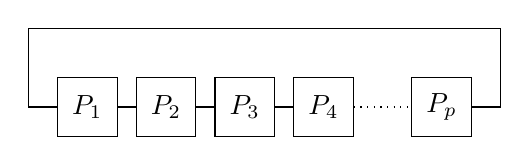
\begin{tikzpicture}
    [
        processor/.style={rectangle, draw, minimum size=5ex},
    ]
    \node (p1) at (1,0) [processor] {$P_1$};
    \node (p2) at (2,0) [processor] {$P_2$};
    \node (p3) at (3,0) [processor] {$P_3$};
    \node (p4) at (4,0) [processor] {$P_4$};
    \node (pp) at (5.5,0) [processor] {$P_p$};
    \draw (p1) -- (p2) -- (p3) -- (p4);
    \draw [dotted] (p4) -- (pp);
    \draw (pp) -- (6.25,0) -- (6.25,1) -- (0.25,1) -- (0.25,0) -- (p1);
\end{tikzpicture}         
                          

            \caption{Netzwerk in Ringform}
        \end{figure}
    \end{columns}
\end{frame}
%----------------------------------------------------------------------%SLIDE -

%----------------------------------------------------------------------%SLIDE -
\begin{frame}
    \frametitle{Netzwerk}
    \framesubtitle{Beispiel: Matrix-Vektor-Multiplikation}
    \begin{columns}[c]
        \begin{column}{0.5\textwidth}
            \begin{equation*}
                A \cdot x =
                \only<1>{
                    \begin{pmat}[{}]
                        a_{11} & a_{12} & a_{13} & a_{14} \cr
                        a_{21} & a_{22} & a_{23} & a_{24} \cr
                        a_{31} & a_{32} & a_{33} & a_{34} \cr
                        a_{41} & a_{42} & a_{43} & a_{44} \cr
                    \end{pmat}
                    \cdot
                    \begin{pmat}[{}]
                        x_1 \cr
                        x_2 \cr
                        x_3 \cr
                        x_4 \cr
                    \end{pmat}
                }
                \only<2->{
                    \begin{pmat}[{|||}]
                        a_{11} & a_{12} & a_{13} & a_{14} \cr
                        a_{21} & a_{22} & a_{23} & a_{24} \cr
                        a_{31} & a_{32} & a_{33} & a_{34} \cr
                        a_{41} & a_{42} & a_{43} & a_{44} \cr
                    \end{pmat}
                    \cdot
                    \begin{pmat}[{}]
                        x_1 \cr\-
                        x_2 \cr\-
                        x_3 \cr\-
                        x_4 \cr
                    \end{pmat}
                }
            \end{equation*}
        \end{column}
        \begin{column}{0.5\textwidth}
            \only<3>{
                \begin{equation}
                    z_i = A_i \cdot x_i =
                    \begin{bmatrix}
                        a_{1i} \\ a_{2i} \\ a_{3i} \\ a_{4i}
                    \end{bmatrix}
                    \cdot
                    \begin{bmatrix} x_i \end{bmatrix}
                \end{equation}
                \begin{equation}
                    A \cdot x = \sum_{i=1}^4 z_i
                \end{equation}
            }
        \end{column}
    \end{columns}
\end{frame}
%----------------------------------------------------------------------%SLIDE -

%----------------------------------------------------------------------%SLIDE -
\begin{frame}
    \begin{algorithm}[H]
        \caption{Asynchronous Matrix Vector Product on a Ring \cite[S.18]{jaja}}
        \begin{algorithmic}[1]
        \Require (1) Prozessor-ID $i$; (2) Anzahl Prozessoren $p$;
        (3) $i$te Submatrix $A_i$
        (4) $i$ter Subvektor $x_i$
        \Ensure $P_i$ berechnet $y = A_1x_1 + \cdots + A_ix_i$
        und gibt das Ergebnis nach rechts. Bei Terminierung hat $P_1$ das
        Ergebnis $z = Ax$.
        \begin{multicols}{2}
            \State Berechne $z_i \gets A_ix_i$
            \If {$i = 1$}
                \State $y \gets 0$
            \Else
                \State \textbf{receive}($y$, left)
            \EndIf
            \State $y \gets y + z_i$
            \State \textbf{send}($y$, right)
            \If {$i = 1$}
                \State \textbf{receive}($z$, left)
            \EndIf
        \end{multicols}
        \end{algorithmic}
    \end{algorithm}
\end{frame}
%----------------------------------------------------------------------%SLIDE -

\subsection{Parallel Random Access Machine}
%----------------------------------------------------------------------%SLIDE -
\begin{frame}
    \frametitle{Parallel Random Access Machine}
    \begin{columns}
        \column{0.5\textwidth}
        \begin{itemize}
            \item \emph{shared memory} Modell
            \item RAMs
            \item gemeinsamer, globaler Speicher
            \item \textbf{global read} und \textbf{global write}
            \item \textbf{pardo} Statement
                \begin{algorithmic}
                    \ParDo {$1 \leq i \leq n$}
                        \State process($i$)
                    \EndParDo
                \end{algorithmic}
        \end{itemize}
        \column{0.5\textwidth}
        \begin{figure}
            \centering
            % PRAM mit p Prozessoren
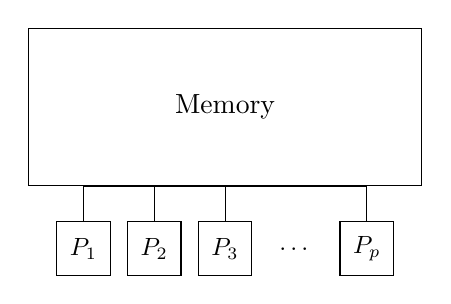
\begin{tikzpicture}
    [
        processor/.style={rectangle, draw, scale=0.9, minimum size=5ex},
        dots/.style={rectangle, scale=0.9, minimum size=5ex},
        scale=0.9,
    ]
    \node (mem) at (3, 2) [
        rectangle,
        minimum height=2cm,
        minimum width=5cm,
        draw,
    ] {Memory};

    \node (p1) at (1,0) [processor] {$P_1$};
    \node (p2) at (2,0) [processor] {$P_2$};
    \node (p3) at (3,0) [processor] {$P_3$};
    \node (p4) at (4,0) [dots] {\ldots};
    \node (pp) at (5,0) [processor] {$P_p$};
    \draw (p1) |- (mem.south);
    \draw (p2) |- (mem.south);
    \draw (p3) |- (mem.south);
    \draw (pp) |- (mem.south);
\end{tikzpicture}         

            \caption{Schema einer PRAM}
        \end{figure}
    \end{columns}
\end{frame}
%----------------------------------------------------------------------%SLIDE -

%----------------------------------------------------------------------%SLIDE -
\begin{frame}
    \frametitle{Parallel Random Access Machine}
    \framesubtitle{Zugriffsbeschränkungen}
    Darf gleichzeitig auf Speicherzellen zugegriffen werden? \\
    Subtypen mit verschiedenen Beschränkungen:
    \begin{description}
        \item[EREW] exclusive read exclusive write
        \item[CREW] \emph{concurrent} read exclusive write
        \item[CRCW] \emph{concurrent} read \emph{concurrent} write
    \end{description}
    \pause
    Was passiert bei gleichzeitigem Schreiben?
    \begin{description}
        \item[common CRCW] Schreibzugriff nur bei übereinstimmendem Wert
        \item[arbitrary CRCW] ein beliebiger Prozessor darf schreiben
        \item[priority CRCW] Zugriff nach Rangordnung
    \end{description}
\end{frame}
%----------------------------------------------------------------------%SLIDE -

%----------------------------------------------------------------------%SLIDE -
\begin{frame}
    \frametitle{Parallel Random Access Machine}
    \framesubtitle{Beispiel}
    \begin{algorithm}[H]
        \caption{Summe \cite[S.26]{jaja}}
        \label{alg:pram-sum}
        \begin{algorithmic}[1]
        \Require $n = 2^k$ Zahlen in einem Array $A$
        \Ensure Die Summe $S = \sum_{i=1}^n A(i)$
        \ParDo {$1 \leq i \leq n$}
            \State $B(i) \gets A(i)$
        \EndParDo
        \For {$h=1$ \textbf{to} $\log n$}
            \ParDo {$1 \leq i \leq n/2^h$}
                \State $B(i) \gets B(2i-1) + B(2i)$
            \EndParDo
        \EndFor
        \State $S \gets B(1)$
        \end{algorithmic}
    \end{algorithm}
\end{frame}
%----------------------------------------------------------------------%SLIDE -
